\documentclass[conference]{IEEEtran}
% If the IEEEtran.cls has not been installed into the LaTeX system files, 
% manually specify the path to it:
% \documentclass[conference]{../sty/IEEEtran} 
\usepackage[brazil]{babel}
\usepackage{amsmath}
\usepackage{multirow}
\usepackage[utf8]{inputenc}
\usepackage[T1]{fontenc}
\usepackage{graphicx}

% correct bad hyphenation here
\hyphenation{op-tical net-works semi-conduc-tor IEEEtran}

\begin{document}
	
	% paper title
	\title{Redes Neurais Artificiais: Revisão da Literatura}
	
	
	% author names and affiliations
	% use a multiple column layout for up to three different
	% affiliations
	\author{\authorblockN{Victor São Paulo Ruela \\}
		\authorblockA{Programa de Pós-Graduação em Engenharia Elétrica\\
			Universidade Federal de Minas Gerais\\
			Belo Horizonte, Brasil\\
            Email: victorspruela@ufmg.br}}
	
	% avoiding spaces at the end of the author lines is not a problem with
	% conference papers because we don't use \thanks or \IEEEmembership
	
	% use only for invited papers
	%\specialpapernotice{(Invited Paper)}
	
	% make the title area
	\maketitle
	
	\begin{abstract}
		Este trabalho tem como objetivo apresentar uma revisão da literatura de redes neurais aritificiais, com enfoque nas evoluções desenvolvidas a partir dos principais trabalhos clássicos, os que estabeleceram os fundamentos desta grande área de pesquisa. 
	\end{abstract}

	\section{Introdução}
	A Rede Neural Artificial (RNA) é uma classe de modelos muito popular em problemas de classificação, reconhecimento de padrões, regressão e predição \cite{jain1996artificial}. Inspirado pelas características do cérebro humano, elas possuem como elementos básicos neurônios artificiais capazes de executar operações matemáticas, representando desta forma modelos de neurônios biológicos. Através de sua organização em diferentes estruturas de rede, tais modelos são capazes de se adaptar e representar funções matemáticas bastante complexas. 
	
	Diferentes representações estão presentes na literatura, as quais são classificadas de acordo com o seu nível de complexidade e requisitos coputacionais de implementação. Hipóteses básicas para regras de aprendizado de associações entre neurônios podem ser encontradas em trabalhos bastante antigos, como abordado no livro de William James em 1982 \cite{james1984psychology}. Entretanto, um grande marco desta área de pesquisa ocorreu na década de 40 após a introdução do modelo de McCulloch and Pitts (MCP) \cite{mcculloch1943logical}, o qual é a adotado atualmente nos principais modelos de RNAs.
	
	O modelo MCP tem como saída a soma das ativações dos neurônios anteriores ponderados pelos pesos das conexões entre eles. Originalmente, uma função de ativação do tipo degrau é aplicada sobre sua saída, configurando modelo de soma-e-limiar originalmente descrito pelos autores. Este trabalho apresentou a configuração de diversas redes de neurônios MCP, com enfoque na implementação de funções lógicas. Vale a pena notar que os primeiros computadores digitais estavam surgindo nesta época, motivando esta aplicação. Entretanto, as estruturas apresentadas eram estáticas e não houve a sugestão de algum método de aprendizado para adaptá-las.
	
	O aprendizado surgiu de forma mais concreta com o postulado de Hebb \cite{hebb2005organization}, originalmente publicado em 1949. De acordo com o autor, a eficiência de uma determinada sinapse que conecta dois neurônios é proporcional à co-ocorrência de ativação entre eles. Portanto, o princípio de aprendizado Hebbiano visa reforçar as conexões relevantes para as diferentes saída da rede, guiado pela correlação entre os neurônios. Considerando o neurônimo MPC, suas primeiras estruturas de rede e algoritmos de treinamento descritos na literatura são o \textit{Adaline} \cite{widrow1960adaptive}, em 1960, e o Perceptron simples, em 1957 \cite{rosenblatt1957perceptron}.
	
	Após um período de euforia com a introdução destes últimos dois modelos, a área de pesquisa de RNAs sofreu um descrédito e frustação até o início dos anos 80. Isso decorreu  do trabalho de Minsky e Papert \cite{minsky1969introduction}, o qual generalizou as limitações destes modelos para problemas considerados fundamentais, como o do OU-exclusivo (XOR). O interesse só foi reativado após o re-descobrimento do algoritmo \textit{back-propagation} para treinamento de redes de múltiplas camadas \cite{rumelhart1985learning}, as quais são capazes de superar as limitações até então existentes das redes de camada única. Destacam-se também a introdução dos mapas de Kohonen \cite{kohonen1982self}, redes recorrentes de Hopfield \cite{hopfield1982neural} e o modelo ART para aprendizado não-supervisionado \cite{carpenter1987massively}. Além disso, nesta época surgiram as primeiras conferências e periódicos dedicados à area de RNAs \cite{macukow2016neural}.
	
	A partir destes princípios elementares, a área de RNAs evoluiu bastante nas últimas décadas. Após a introdução das primeiras regras de aprendizado, este tipo de modelo ganhou maior visibilidade e aplicabilidade para problemas reais, sendo possível encontrar uma enorme quantidade de aplicações publicadas \cite{abiodun2018state}. Além disso, o aumento dos recursos computacionais disponíveis fomentou o desenvolvimento de novas técnicas para aprendizado e o aprimoramento das existentes, além de propostas de novas estruturas redes complexas capazes de lidar com problemas de grande dificuldade.
	
	Portanto, o objetivo deste trabalho é apresentar a uma revisão da literatura contendo os principais trabalhos e entender a evolução dos diferentes modelos de redes neurais utilizadas atualmente. Partindo das referências clássicas, diferentes abordagens propostas serão analisadas de forma cronológica com o intuito de se entender a evolução desta área de pesquisa até o tempo presente. Este trabalho será divido da seguinte forma: a Seção II apresenta uma revisão da literatura com uma análise crítica dos principais trabalhos, os quais serão organizados usando como referência o livro de Simon Haykin \cite{haykin2007neural} e as notas de aula. Na seção III serão apresentadas algumas das principais aplicações de RNAs publicadas. Finalmente, é feita uma conclusão deste trabalho.
		
	
%	\subsection{Problemas de classificação}
%	A tarefa de classificação consiste em associar um conjunto de padrões de entrada, representado por um vetor de características, para uma de varias classes previamente definidas.

%	\subsection{Problemas de regressão}
%	Dado um conjunto de $N$ pares de dados de entrada-saída $\left\lbrace (\mathbf{x}_1, y_1), \dots, (\mathbf{x}_N, y_N)\right\rbrace$, o objetivo da regressão é encontrar uma função aproximada $\hat{f}(\mathbf{x})$ que melhor descreve a função desconhecida $f(\mathbf{x})$ utilizada para gerar estes dados.
%
%	\subsection{Problemas de predição}
%	Considerando um conjunto de $N$ $\left\lbrace y(t_1),\dots, y(t_N) \right\rbrace $ amostras ordenadas em função do instande de tempo em que foram amostradas $t_1, \dots, t_N$, o objetivo da predição é estimar qual será o valor da amostra $y_{N+1}$ em um tempo futuro $t_{N+1}$.
%
%	\subsection{Problemas de reconhecimento de padrões}
	
	\section{Revisão da Literatura}
	%RNAs de aprendizado supervisionado são responsáveis pela inferência de uma função desconhecida $f(.)$ que realiza o mapeamento entre uma saída e um conjunto de entradas medidas, representada pelo conjunto de $N$ pares de dados $\mathcal{D} = \left\lbrace (\mathbf{x}_1, y_1), \dots, (\mathbf{x}_N, y_N)\right\rbrace $. Problemas de classificação e regressão são comumente solucionados com estas técnicas, para os quais as primeiras estruturas de rede e algoritmos de treinamento descritos na literatura são o \textit{Adaline}, em 1960, e o Perceptron simples, em 1957. 
	
	\subsection{Aprendizado Hebbiano}
	

	\subsection{Perceptron}
	Proposto inicialmente por Rosenblatt \cite{rosenblatt1957perceptron}, este é um modelo geralmente utilizado para a solução de problemas de classificação. No seu trabalho original, o autor descreve formas de adaptação dos parâmetros, ou pesos, da rede com o objetivo de reduzir a discrepância entre as saídas esperadas e estimadas e aprender associações entre os neurônios, o que é a base da indução para diversos algoritmos atuais. Este trabalho é considerado um marco na literatura por diversos autores. Embora descrito como uma rede de duas camadas, originalmente seu treinamento só considerava uma camada. Por esse motivo, o Perceptron simples é comumente descrito na forma de somente um neurônio MCP. Sua regra de aprendizado é bem direta e consiste em alterar iterativamente os pesos da rede adicionado o erro total entre as saídas medidas estimadas ponderada pelo vetor de entradas \cite{haykin2007neural}. 
	
	Se considerarmos uma função de ativação contínua e diferenciável, os pesos da rede poderão ser inferidos de forma explícita, através do cálculo da pseudo-inversa, ou pelo algoritmo do gradiente descendente \cite{hertz1991introduction}. Exemplos de funções de ativação com esta característica frequentemente empregadas na literatura são a função logística, tangente hiperbólica e linear \cite{jain1996artificial}. Vale a pena ressaltar que a covergência destas abordagens está condicionada aos dados utilizados para treinamento serem linearmente independentes \cite{hertz1991introduction}.
	
	Rosenblatt provou a convergência da regra de aprendizado original, porém a mesma só é garantida para problemas linearmente separáveis, o que constitui a principal limitação deste modelo. O trabalho de Minsky e Papert \cite{minsky1969introduction} evidenciou bastante esta limitação e através da aplicação do Perceptron a diversos problemas considerados fundamentais, levou ao descrédito deste modelo pela comunidade científica. Após este trabalho, Rosenblatt avaliou diferentes arquiteturas de rede tentando superar esta limitação, mas não conseguiu chegar ao desenvolvimento do aprendizado para múltiplas camadas. Por conta disso, o Perceptron foi pouco estudado pelos próximos de 20 anos \cite{hertz1991introduction}.
	
	O interesse pelo Perceptron retornou na década de 80 com a descrição do método de aprendizado conhecido como \textit{back-propagation}, o qual é capaz de aprender os pesos de redes de múltiplas camadas de forma eficiente \cite{rumelhart1985learning}. Aliado a isso, o Perceptron de múltiplas camadas é capaz de descrever superfícies de separação não-lineares, superando a pricipal limitação do trabalho de Rosenblatt. Uma descrição mais completa desta família de modelos é feita na próxima seção.

	\subsection{Adaline}
	O Adaline foi inicialmente desenvolvido por Widrow em 1960 \cite{widrow1960adaptive}, sendo principamente aplicado em problemas de regressão lineares. Assim como o Perceptron, originalmente este modelo considera somente um neurônio MCP em sua formulação, entretando sua função de ativação é a identidade. Seu treinamento é formulado como um problema de otimização com custo quadrático, onde originalmente foi utilizado o algoritmo do gradiente descendente para sua solução. 
	
	Para este agoritmo, em cada iteração é dado um passo na direção oposta ao gradiente da função objetivo, resultanto em uma convergência gradual para o mínimo do problema. Este gradiente pode ser calculado de forma análitica para a estrutura de rede do Adaline, o qual é no fim proporcional à diferença entre os valores estimados e reais \cite{widrow1960adaptive}, bastante similar ao Perceptron simples. É fácil notar que o treinamento também pode ser realizado de forma direta através do cálculo da  pseudo-inversa dos dados de entrada, já que este é um problema de mínimos quadrados \cite{haykin2007neural}.
	
	Uma extensão proposta deste modelo é conhecida como Madaline, o qual é caracterizada por uma rede composta por vários Adalines. Existem duas principais regras para seu treinamento, conhecidas por MRI \cite{widrow1962generalization} and MRII \cite{winter1988madaline}. É interessante notar que a MRI surgiu bem antes do algoritmo \textit{back-propagation}, podendo ser considerada uma estrutura primitiva de uma rede de múltiplas camadas. Os leitores são referidos à \cite{widrow199030} para uma descrição mais completa destas regras e suas aplicações.
	
	   
	
	 
	
%	, possuindo uma estrutura neural similar usualmente referida ao um filtro adaptivo. Essa característica vêm do fato do processo de aprendizagem ser separado em duas fases: (1) Geração de dois sinais intermediários, correspondendo ao sinal de saída estimada e outro de erro; (2) adaptação dos pesos do neurônio de acordo com o sinal de erro \cite{haykin2007neural}.
		
	\subsection{Perceptron de múltiplas camadas}
	
	O Perceptron de múltiplas camadas (MLP) é uma rede neural com uma ou mais camadas escondidas, ou seja, localizadas entre as entradas e saídas do modelo. Além disso, são caracterizadas por um alto grau de conectividade e por aplicar funções de ativação não-lineares e diferenciáveis ao modelo dos neurônios \cite{haykin2007neural}. Estas camadas adicionais funcionam como detectores de características, aplicando transformações não-lineares sequenciais aos dados de forma que estes sejam mais facilmente separados nesse novo espaço. Portanto, a introdução das camadas escondidas permite modelar superfícies de decisão não-lineares, sendo consideradas aproximadores universais de funções se a função de ativação é contínua, limitada e não-constante  \cite{hornik1989multilayer}.
		
	O treinamento de redes de camada única vistas nas seções anteriores é bem direto pois podemos facilmente derivá-las analiticamente. Entretando, ao incluir camadas escondidas e alta conectividade, analisar teoricamente o comportamento do Perceptron torna-se mais difícil. Aliado a isso, o seu treinamento se torna mais complexo justamente por haver uma maior quantidade de estruturas de rede possíveis para representar os dados de entrada. O primeiro algoitmo eficiente de treinamento de tais foi formalizada por Rumelhart em 1985 \cite{rumelhart1985learning}, conhecido como \textit{back-propagation}.    
	
	O \textit{back-propagation} é uma técnica de aprendizado online (ou estocástica), na qual os pesos da rede são ajustados amostra-a-amostra. Ou seja, em cada época de treinamento, os dados de entrada são apresentados individualmente para a rede objetivando a minimização do erro das saídas estimadas e desejadas. O algoritmo pode ser dividido em duas etapas: na primeira os dados são apresentados à rede mantendo os pesos fixos, e calculada a sua respectiva saída; na segunda, o sinal de erro em relação à saída esperada é calculado e propagado no sentido inverso da rede, onde ajustes sucessivos são realizados. A atualização dos pesos da rede é feita com base na técnica do gradiente descendente, cuja derivação completa será omitida deste trabalho por brevidade. O leitor pode encontrá-la em \cite{rumelhart1985learning, haykin2007neural}. 
	
	Embora bastante eficiente, sua convergência pode ser lenta se o algoritmo não for usado corretamente \cite{lecun1993efficient}. É recomendado realizar a normalização das entradas para equalizar a taxa de atualização dos pesos entre as camadas, além de remover variávies altamente correlacionadas \cite{lecun2012efficient}. Ainda de acordo com \cite{lecun2012efficient}, é sugerido o uso de sigmoides simétricas, como a tangente hiperbólica, as quais geralmente possuem maior velocidade de convergência. Além disso, é importante que os valores desejados estejam dentro dos limites da sigmoide escolhida. Outro fator importante é a taxa de treinamento: \cite{magoulas1999improving} apresenta o estudo de algumas técnicas para adaptação da taxa de treinamento presentes na literatura, mostrando que o seu uso é bastante benéfico. 
	
	É interessante notar que os problemas descritos anteriormente são similiares aos encontrados para a otimização de funções não-lineares e não-convexas. Ou seja, é possível analisar o treinamento do MLP como um problema de otimização e aplicar diferentes algoritmos e heurísticas disponíveis da literatura. De fato, isso é explorado por diversos autores, os quais aplicam o método de Newton \cite{becker1988improving}, gradiente conjugado \cite{johansson1991backpropagation}, Gauss-Newton \cite{battiti1992first}, Levenberg-Marquardt \cite{hagan1994training} e Quasi-Newton \cite{robitaille1996modified}.  
	
	Métodos de segunda ordem possuem o atrativo da convergência acelarada, mas em contra-partida é necessária a estimativa da Hessiana, o que exige mais recursos computacionais e está sujeito a problemas numéricos adicionais, sendo limitado a redes pequenas e a usar usando aprendizado por batelada. Portanto, este são fatores que devem ser levados em conta na hora de escolher o otimizador para realizar o treinamento de uma rede. Conforme argumentado por \cite{lecun2012efficient}, o uso de informações de segunda ordem nem sempre é necessário em alguns problemas, para os quais a técnica do gradiente estocástico bem ajustada é dificilmente superado para problemas de larga escala.
	
	O estado da arte para treinamento de RNAs são o algoritmo Adadelta \cite{zeiler2012adadelta} e o Adam \cite{kingma2014adam}, impulsionado pelo crescimento da popularidade das redes de aprendizado profundo. 
	
	
	Mais recentementes, alguns autores começaram a propor o uso de algoritmos evolucionários (EAs) para o treinamento do MLP. Eles são atrativos pelo fato de convergirem para o ótimo global se um tempo de treinamento suficiente estiver disponível. Entretanto, o custo computacional poderá ser bastante alto, além do ajuste dos hiper-parâmetros ser trabalhoso. Em \cite{ilonen2003differential}, os autores propõe o uso do algotimo Differential Evolution, o qual concluem que ele não apresenta desempenho superior ao \textit{back-propagation}. Já \cite{ding2011optimizing} propôs uma técnica híbrida de algoritmos genéticos e backpropagation, a qual se mostrou menos suscetível a ficar presa em mínimos locais durante o treinamento. O leitor pode ser referir a \cite{mirjalili2019evolutionary} para um estudo mais completo de EAs e RNAs. Outro área interessante são as redes neurais evolutivas \cite{yao1999evolving}, para as quais além do treinamento dos pesos evolui-se também outras características da rede.
	
	\subsection{Redes de funções de base radial (RBF)}
	As redes RBF foram inicialmente introduzidas por \cite{broomhead1988multivariablefi} e são caracterizadas por um aprendizado que envolve duas etapas: (i) aplicar uma transformação aos padrões para um espaço onde a expecativa de serem linearmente separáveis é alta (ii) encontrar os pesos usando o estimador mínimos quadrados usado no Perceptron simples. Essa estrutura pode ser representada por um rede de três camadas, onde sua camada escondida é reponsável pela transformação não-linear das estradas para o novo espaço, geralmente para uma dimensão muito alta. 
	
	Essa transformação é justificada pelo teorema de Cover sobre a separabilidade de padrões \cite{cover1965geometrical}, o qual diz que um problema de classificação complexo projetado não-linearmente para um espaço de alta dimensão é mais provável de ser separável do que em um espaço de baixa dimensão, desde que o espaço não seja densamente povoado. Boa parte da teoria, que é relacionada ao campo de interpolação multivariável, considera um kernel baseado na função Gaussiana, que é uma classe importante de RBFs. Teoricamente, as redes RBF podem ser consideradas um aproximador universal de funções contínuas se a RBF é selecionada apropriadamente \cite{poggio1990networks, park1991universal, liao2003relaxed}. Uma condição apropriada é dada pelo teorema da interpolação de Miccchelli \cite{micchelli1986interpolation}, ou quando uma determinada classe de RBFs é contínua e diferenciável \cite{park1991universal}, por exemplo.
	 
	No seu treinamento, além de tratamentos especiais na presença de ruídos nos dados \cite{broomhead1988radial}, uma etapa importante é a estimativa dos parâmetros das unidades Gaussianas além dos pesos da rede. Isso pode ser feito distribuindo os centros uniformemente, por exemplo. De forma mais geral, pode-se selecionar aleatoriamente subconjutos dos padrões de entrada se este são representativos e grandes o suficiente para o apredizado \cite{wu2012using}. Para aproximação de funções, uma heurística possível é colocar os centros nos extremos da derivada de segundo grau da função e também mais densamente em áreas cujo valor absoluto e maior \cite{sanchez1995second}, o que possui resultados melhores em relação à distribuição uniforme.
	
	Outra abordagem bastante utilizada para a definição dos centros é o uso de técnicas de agrupamento (\textit{clustering}) dos dados presentes na literatura \cite{du2006neural, du2010clustering}.  Uma escolha popular são o algoritmo não-supervisionado \textit{k-means} \cite{moody1989fast} e redes neurais baseadas em memórias associativas \cite{kohonen2012self}. Também podem ser utilizadas técnicas de clustering supervisionadas \cite{chen1993hybrid}, as quais podem ser mais eficientes para redes RBF \cite{wu2012using}. Após determinados os centros, define-se as matrizes de convariância das RBFs como a convariância dos dados de cada \textit{cluster} \cite{wu2012using}. 
	
	Com os centros e covariâncias definidos, o aprendizado dos pesos é feito pela minimização do erro quadrático médio. Para problemas simples, pode-se utilizar o algoritmo de mínimos quadrados ou gradiente descendente, similar ao aprendizado do Perceptron simples. O treinamento via gradiente descendente é equivalente ao do MLP \cite{wettschereck1992improving}, onde pode-se também utilizar as mesmas abordagens por otimização irrestrita \cite{du2006neural}.	Uma descrição de diferentes abordagens para treinamento de RBFs por otimizaçao podem ser encontradas em \cite{wu2012using}, como o uso de \textit{back-propagation} seletivo \cite{vakil2004training} e programação linear \cite{roy1995algorithm}.
	
	No caso dos mínimos quadrados, problemas complexos que requerem um número elevado de RBFs na camada escondida estão sujeitos a problemas numéricos na estimativa da pseudo-inversa. Para lidar com isso, uma abordagem comum é o uso de técnicas de ortogonalização, como as decomposições SVD e QR \cite{golub1980analysis}. Em algumas condições, é possível também resolver esse problema usando a transformada de Fourier da rede RBF, a qual requer menos esforço computacional necessário \cite{abe2003fast}. Outra alternativa eficiente é aplicar a ortogonalização de Gram-Schimidt (GSO) à RBF \cite{kaminski1997kernel}, a qual possui menor requisito de armazenamento e pode sem implementado de forma paralela.
	
	Outra forma eficiente para aprendizado da rede consiste no uso da técnica de mínimos quadrados ortogonal (OLS) \cite{chen1991orthogonal, chen1992orthogonal, chen1995fast, hong1997givens}. Nesta abordagem, não só os pesos podem ser determinados, mas também a quantidade e centros das RBFs. o GSO é inicialmente aplicado para contruir um conjunto de vetores ortogonais no espaço criado pela unidade escondida, e na sequência um novo centro RBF é selecionado de acordo com a sua minimização do erro quadrático médio de treinamento. Esse algotimo pode ser executado de forma sequencial ou reversa, ou seja, podemos iniciar com uma rede vazia ou com o máximo de unidades escondidas, por exemplo. Existem também versões recursivas deste algoritmo na literatura, conhecidas por ROLS \cite{yu1997recursive}, as quais são aplicadas a problemas envolvendo sistemas de múltiplas entradas e saídas, por exemplo.
	

	\subsection{Generalização}
    Uma das suas principais características do modelo RNA é sua habilidade de generalização, que é sua capacidade em estimar corretamente dados ainda não vistos. Em outras palavras, algoritmos de aprendizado de RNA possuem como objetivo encontrar um modelo que consigar caputar as principais características do conjunto de dados de treinamento, mas que também seja capaz de prever com precisão um conjunto de teste ainda não visto.
        
    Este conceito é introduzido pela primeira vez por Geman et. al em 1992 \cite{geman1992neural}, o qual é o bastante conhecido dilema viés-variância. Através deste trabalho, os autores introduzem o conceito de que existe uma competição entre duas fontes de erro que impede o modelo de generalizar além dos dados de treinamento, o viés e a variância. Além disso, eles mostra que existe um compromisso entre estas grandezas, de forma que quando um modelo com viés máximo possuirá mínima variância, e vice-versa.
    
    O erro de viés está relacionado a suposições incorretas sobre o modelo, podendo ser defindo como a diferença entre o valor previsto médio e o esperado. Um alto viés leva ao fenômeno de \textit{under-fitting}, onde o modelo possuem uma estrtura simples e não é capaz de representar os principais padrões presentes nos dados. Já o erro de variância indica a sensibilidade do modelo a flutuações no conjunto de treinamento. Uma variância elevada leva ao fenômeno de \textit{over-fitting}, onde o modelo é bastante complexo que se ajusta perfeitamente aos dados de treinamento. Um exemplo deste comportamente pode ser visto na Figura \ref{fig:bias-var}. É importante notar que estes dois erros podem contribuir para um desempnho ruim, ou seja, mesmo um modelo não-enviésado com variância alta pode resultar em um erro de treinamento maior que o esperado \cite{geman1992neural}.
    
    \begin{figure}[thpbh]
    	\centering
    	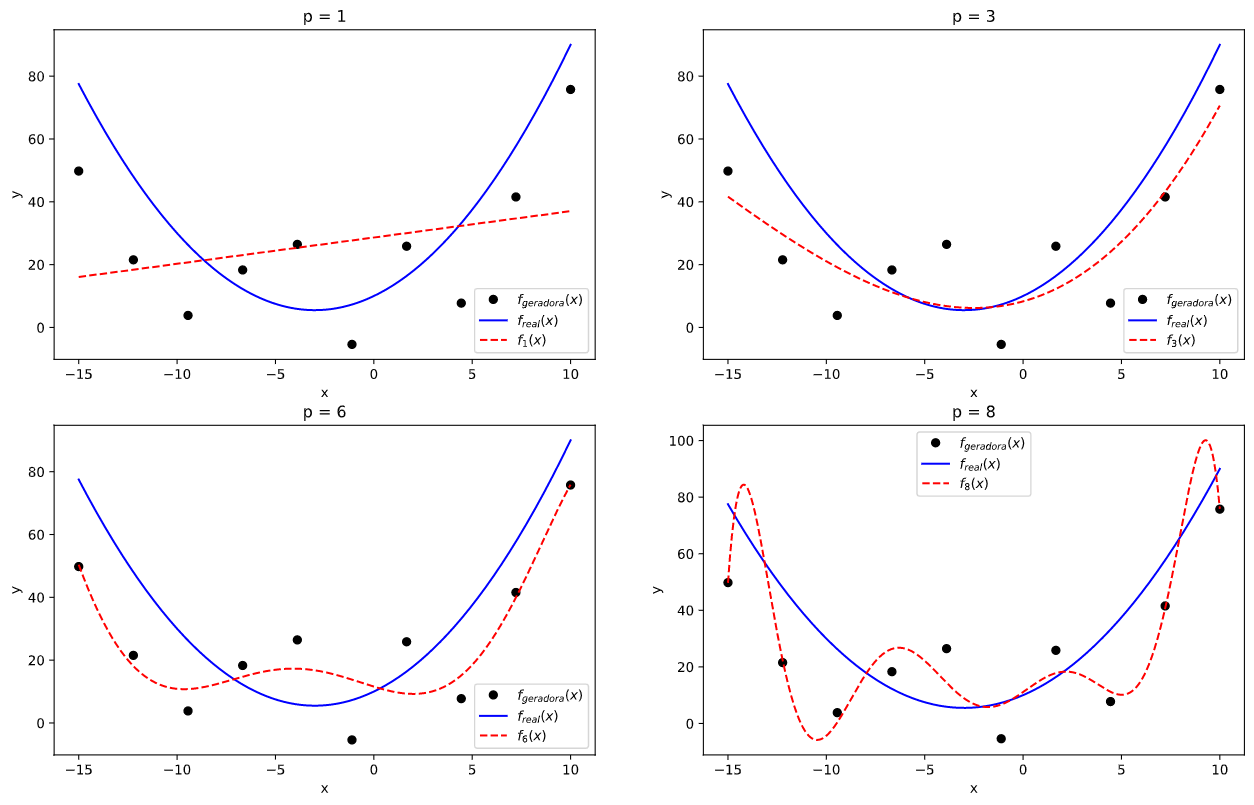
\includegraphics[width=0.5\textwidth]{bias-var-example.png}
	    \caption{Exemplo de \textit{under-fitting} ($p=1$) e \textit{over-fitting} ($p > 3$) para problema de regressão polinomial sobre dados uma função quadrática.}
	    \label{fig:bias-var}
    \end{figure}
    
	Existem algumas formas de se balancear o viés e variância, as são divididas no caso da conjuntos amostras finitas e asintóticamente infinitas. Por serem mais comuns em aplicações práticas, as últimas serão omitidas deste trabalho e o autor pode se referir a \cite{geman1992neural} para mais detalhes. Para conjuntos de dados finitos, destacam-se a validação cruzada \cite{arlot2010survey} e o uso de regularização pela inclusão de penalidades à função objetivo do treinamento \cite{girosi1995regularization}.  
	
	O conceito de generalização deu origem a técnicas de aprendizado que incluem em sua formulação formas de se balancear o viés e a variância automaticamente. Entre eles, destacam-se as máquinas de vetores suporte (SVM), máquinas de aprendizado extrem (ELM)  e o aprendizado multiobjetivo.
	
	\subsection{Máquinas de aprendizado extremo}
	Inicialmente proposto por \cite{huang2004extreme}, as máquinas de aprendizado extremo (ELM) são redes neurais \textit{feed-forward} com uma única camada escondida, as quais possuem o atrativo de poucos parâmetros a serem ajustados, generalização maior ou similar e redução do tempo de treinamento das redes em relação aos métodos convencionais. Seu treinamento é baseado na teoria de minimização de risco empírico, necessitando de somente uma iteração para este processo, evitando múltiplas iterações e algoritmos de otimização local \cite{ding2015extreme}. 
	
	ELMs são capazes de definir adaptivamente o número neurônios da rede e aleatoriamente escolher os pesos das entradas e viéses da camada escondida \cite{huang2006extreme}. Isso faz com o que a rede possa ser considerada como um sistema linear, o qual pode ser calculado de forma analítica através de uma operação de inversão da matriz de pesos da camada de saídas \cite{huang2006extreme}. Essa característica permite uma drástica redução do esforço computacional do treinamento, geralmente de 10 vezes ou mais \cite{deng2010research}. 
	
	Apesar do apelo no ganho de tempo de treinamento, essa abordagem permite menor adaptabilidade ao conjunto de dados, além de problemas numéricos para o cálculo da inversão por mínimos quadrados e problemas de robustez se os dados forem ruidosos \cite{ding2015extreme}. Além disso, a aleatoriedade na  escolha de pesos e viéses pode levar a uma quantidade maior de neurônios na camada escondida, bem como tornar o sistema linear não solucionável e reduzir sua acurácia \cite{wang2011study}.
	
	Embora tenha sido proposto bem recentemente (2004), têm recebido uma atenção considerável na literatura a nível téorico e de aplicações \cite{huang2011survey}. Do ponto de vista da teoria, o foco dos autores é divido entre duas frentes: (1) aprimorar sua capacidade universal de aproximação com camadas escondidas aleatórios e (2) propor novas técnicas de aprendizado mais rápidas e robustas. De acordo com uma revisão feita em 2011 por Huang et. al  \cite{huang2011survey}, destacam-se o ELM baseado em kernel \cite{huang2011extreme},  ELM com aprendizado online \cite{liang2006fast, zhang2018survey}, ELM incremental \cite{huang2008enhanced}, \textit{ensemble} de ELM \cite{sun2008sales, van2009adaptive, lan2009ensemble} e ELM com poda \cite{rong2008fast}.
	
	   
    
	\subsection{Máquinas de vetores suporte}
	Introduzido por Vapnik em 1992 \cite{boser1992training} ás máquinas de vetores suporte (SVM) são considerados um dos algoritmos mais robustos e poderosos para aprendizado supervisionado até os dias atuais. No trabalho de Vapnik, o autor apresenta de forma bem completa os fundamentos teóricos deste modelo, apresentando justificativas para sua ótima capacidade de generalização, bem como os limites para a sua validade. Seu princípio de treinamento está na maximização da margem entre os padrões de treino e a superfície de decisão, que é uma representação convexa do compromisso entre viés e variância.
	
	Estas propriedades são uma consequência do uso dos chamados vetores de suporte no seu treinamento, que são os sub-conjuntos de dados mais próximos da superfície de decisão, ou seja, os mais difícies de classificar e relevantes para sua otimalidade. O problema então consiste em encontrar o hiperplano que maximiza a margem de separação entre os padrões, que é equivalente a minimizar a norma Euclidiana do seu vetor de pesos \cite{haykin2007neural}. Isso pode ser visto graficamente na Figura \ref{fig:svm}.
	
	\begin{figure}[thpbh]
		\centering
		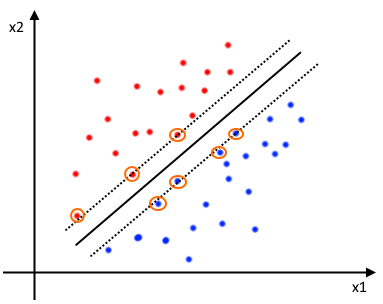
\includegraphics[width=0.3\textwidth]{svm-hp.png}
		\caption{Elementos principais da otimização pela maximização da margem. Para um problema de classificação binário, é encontrado o hiper-plano separador (linha sólida) que maximiza a distância dos vetores de suporte (pontos marcados em laranja). As linhas pretas pontilhadas representam os hiper-planos de suporte.}
		\label{fig:svm}
	\end{figure}
	
	O problema de encontrar o vetor de pesos que define o hiper-plano foi convenientemente formulado com base na teoria de otimização convexa. Isso é muito importante pois esta classe de problemas tem sua otimalidade garantida e bem definida, não estando sujeita aos problemas observados no algoritmo \textit{back-propagation}, por exemplo. A função objetivo é descrita como a norma Euclideana dos pesos somada acrescida um segundo termo que limita a quantidade de erros de treinamento, já que os dados podem não ser perfeitamente serparáveis por um hiper-plano. Este problema é então transformado utilizando a técnica de multiplicadores de Lagrange, a qual faz com que seja descrito em função somente dos dados de treinamento.
	
	O segundo termo pode ser ajustado pelo usuário por meio de uma constante, a qual irá controlar o nível de regularização aplicada ao problema, o que resulta em sua característica de generalização. Um valor alto poderá resultar em \textit{over-fitting} se os dados forem ruidosos, o que sugere cuidado na sua escolha.	Sua definição pode ser feita experimentalmente usando técnicas de validação cruzada \cite{arlot2010survey}, por exemplo.
	
	Através da discussão anterior, é fácil notar que o SVM é aplicável somente a problemas linearmente separáveis se são for realizada nenhuma transformação não-linear aos dados. Portanto, um conceito importante utilizado por este algoritmo são os \textit{kernels} \cite{shawetaylor2004kernel}. A partir da escolha de um kernel apropriado \cite{mercer1909xvi,courant89}, o problema poderá ser resolvido por um modelo linear. Note que isto é bem similiar ao princípio de funcionamento das redes RBF. Em relação ao MLP, ele possui a vantagem de controlar a complexidade independente de sua dimensionalidade, ou seja, é possível ter uma quantidade muito grade de neurônios na camada escondida, conforme o teorema de Cover \cite{cover1965geometrical}, e ainda assim obter uma boa generalização \cite{scholkopf2018learning}. 	Um diagrama mostrando o algotimo SVM completo pode ser visto na Figura \ref{fig:svm-completo}.
	
	\begin{figure}[thpbh]
		\centering
		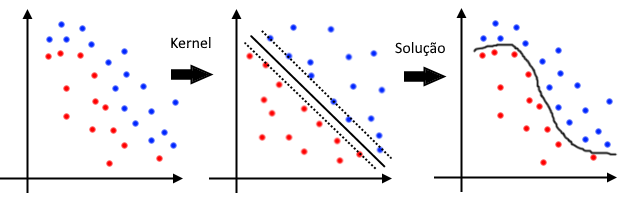
\includegraphics[width=0.5\textwidth]{svm-completo.png}
		\caption{Diagrama do algoritmo SVM}
		\label{fig:svm-completo}
	\end{figure}
	
 	Embora muito poderoso, esse algoritmo é caracterizado por um elevado custo computacional de sua implementação \cite{bottou2007support}. Como sua complexidade pode ser proporcional ao quadrado da quantidade de amostras de treinamento, sua aplicação em problemas de grande porte pode se tornar proibitiva. Outra limitação está relacionada à solução do problema de otimização, uma vez que solvers disponíveis possuem suas próprias limitação em relação ao número de variáveis de decisão suportadas. O problema de otimização é ainda mais dificultado pela esparsidade da solução do SVM, pois o vetor de pesos a ser encontrado possuirá poucos elementos não-nulos \cite{haykin2007neural}, resultando em problemas númericos que impedirão sua correta solução. Diversas melhorias foram propostas para melhorar esta situação, as quais são classificadas entre seleção de dados \cite{wang2005training}, decomposição \cite{dong2005fast}, geometria \cite{zeng2008geometric}, implementação paralela \cite{graf2004parallel} e heurísticas \cite{decoste2000alpha}.
 	
 	Outra limitação deste algoritmo está relacionada a dados não-balanceados. Técnicas propostas para lidar com essa situação realizam o balanceamento dos dados antes do treinamento, ou modificam a estrutura do modelo para torná-los menos sensitivos. As técnicas mais comuns são o \textit{under} e \textit{over-sampling}, e o SMOTE \cite{chawla2002smote}. Esta última é mais indicada para SVMs \cite{chawla2003smoteboost}. É importante ressaltar também que o SVM foi originalmente formulado problemas de classificação binária, de forma que este precisou de ser posteriormente extendido para ser aplicação à essa classe de problemas \cite{weston1998multi, liu2005one}.
 	
	
	Em \cite{cervantes2020comprehensive}, os autores apresentam um revisão bem completa da literatura de SVMs para classificação. Embora utilizado com sucesso em diversas aplicaçõos reais, o SVM ainda possui pouca adoção para problemas com grandes volumes de dados, bem como baixo desempenho para dados não-balanceados. Como tendências de trabalhos futuros, os autores citam além de melhorias nestes problemas clássicos, avanções em treinamento on-line, seleção automática de kernel e parâmetros com menor custo, além de aplicações para aprendizado semi-supervisionado.
	
	\subsection{Aprendizado multiobjetivo}

	\subsection{SOM}
	
	\section{Aplicações}
	
	\section{Conclusões}

%	\section{Aprendizado semi-supervisionado}

%	\section{Generalização}
%	 Uma das suas principais características do modelo RNA é sua capacidade de generalização.  Em geral, algoritmos de aprendizado supervisionado possuem como objetivo minimizar o erro quadrático dos valores previstos pelo modelo em relação às saídas em estudo:
%	 \begin{equation}
%	 	\sum_{i=1}^{N} [y_i - f(\mathbf{x}_i)]^2
%	 	\label{eq:sqrd}
%	 \end{equation}
%	 onde $y_i$ é uma resposta desejada para uma entrada $\mathbf{x}_i$, e $f$ é o função que aproxima a resposta desejada. Ou seja, estamos interessados em encontrar o conjunto de pesos $\mathbf{w}$ da rede a partir dos pares de dados de entrada-saída $\mathcal{D} = \left\lbrace (\mathbf{x}_1, y_1), \dots, (\mathbf{x}_N, y_N)\right\rbrace $ que melhor aproxima a função desconhecida $f$.
%	 
%	 Entretanto, se os dados a serem modelados são ruidosos o uso deste único objetivo pode levar a um overfitting sobre o conjunto de dados de treinamento, de forma que este não consiga generalizar bem para novos valores observados. Estatisticamente, podemos definir a efetividade de $f$ como um estimador de $y$ como \cite{geman1992neural}:
%	 
%	 \begin{equation}
%	 	\begin{aligned}
%	 		E[(y - f(\mathbf{x}; \mathcal{D}))^2 | \mathbf{x}, \mathcal{D}] \quad = & \quad E\left[ (y - E \left[ y | \mathbf{x}\right] )^2 | \mathbf{x}, \mathcal{D}\right]   \\
%	 		& \quad + (f(\mathbf{x};\mathcal{D}) - E[y|\mathbf{x}])^2
%	 	\end{aligned}
%	 \end{equation}
%	 
%	 É importante notar neste indicador que o primeiro termo representa a variância de $y$ dado $\mathbf{x}$, não dependendo dos dados. Já o segundo termo mede a distância entre o estimador e a regressão. Logo, podemos definir o error quadrático médio de $f$ como um estimador da regressão $E[y|\mathbf{x}]$ para um conjunto de dados $\mathcal{D}$ como:
%	 
%	 \begin{equation}
%	 	\begin{aligned}
%	 		& E_{\mathcal{D}}[(f(\mathbf{x};\mathcal{D}) - E[y|\mathbf{x}])^2] = \\ 
%	 		& \qquad \qquad \qquad (E_{\mathcal{D}}[f(\mathbf{x}; \mathcal{D})] - E[y|\mathbf{x}])^2 \quad \text{``viés''} \\
%	 		& \qquad \quad  + E_{\mathcal{D}}\left[ f(\mathbf{x};\mathcal{D}) - E_{\mathcal{D}}[f(\mathbf{x};\mathcal{D})]\right]   \quad \text{``variância''}
%	 	\end{aligned}
%	 \end{equation}
%	 A derivação completa da relação acima pode ser encontrada em \cite{geman1992neural}. Logo é fácil notar que o aprendizado de RNAs é um problema multi-objetivo, no qual precisamos encontrar uma solução de compromisso entre o viés e a variância do modelo. Portanto, em um dos extremos teremos um conjunto de pesos que resultam em um viés máximo (\textit{underfitting}) e no outro variância máxima (\textit{overfitting}).

	
    \bibliographystyle{unsrt}
	\bibliography{survey}
	
\end{document} 